\chapter{Demonstrative Experiment}
\label{chapter:demonstrative-experiment}

This chapter presents a demonstrative simulation experiment done on the CN6880 PSE model. The goal of the experiment is to demonstrate how the queue types and priorities affect the scheduler, and hence the packet throughput and latency, and at the same time validate the scheduler functionality implemented in the model. It also demonstrates the usage of probes to detect bottlenecks in a system.

\section{Experiment Setup}
\label{sec:experiment-setup}

The experiment consists of two different simulations and measurements. We will first demonstrate a packet processing application whose throughput is limited due to the bottleneck occurring from a slow atomic processing. We will then modify the application, splitting part of the atomic processing into parallel, thus breaking the bottleneck.

The simulation consists of a single packet stream, which is generated from a two level workload model. The first workload node is similar workload generator node as presented in Figure~\ref{fig:full-model}. It trigger its child node with interval $RNS\_random\_uniform(5e^{-5}, 15e^{-5})$ seconds, and lifetime of 0.05 seconds. The child node creates 512B packets with interval $5.1e^{-8}$ * $RNS\_random\_lognormal(-10, 0.9)$ seconds for $4e^{-5}$ seconds.

The first packet processing application is shown in the Figure~\ref{fig:application-1}. It consists of two processing steps, each consuming CPU and memory for the range of 5000 clock cycles. The first step consists of parallel, priority 2 queue, and the second one is done atomically with priority 1 queue.

\begin{figure}[]
  \begin{center}
    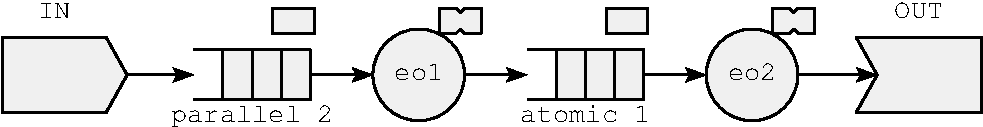
\includegraphics[width=\textwidth]{images/application-1.pdf}
    \caption{The example application used for the experiment. The atomic queue of eo2 produces a bottleneck to the system.}
    \label{fig:application-1}
  \end{center}
\end{figure}

In the second simulation application, presented in Figure~\ref{fig:application-2}, we will use a modified packet processing application, where the second processing step shown in Figure~\ref{fig:application-1}, is split into parallel and atomic steps.

\begin{figure}[]
  \begin{center}
    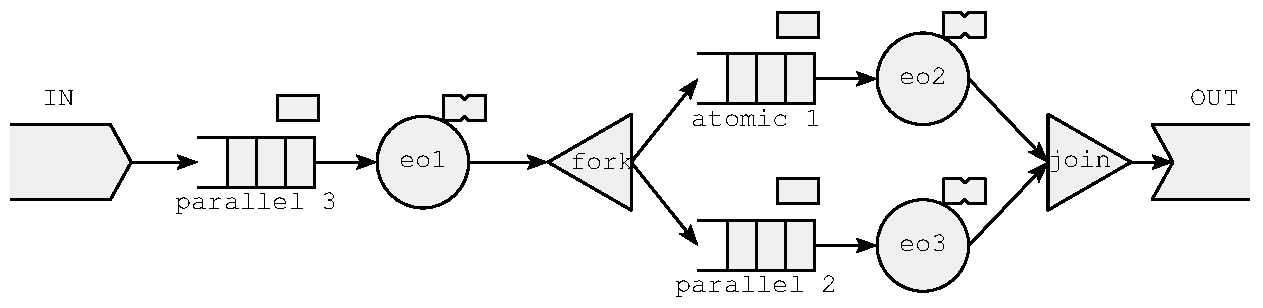
\includegraphics[width=\textwidth]{images/application-2.pdf}
    \caption{A modified processing application for the experiment. The bottleneck has been removed by splitting the second processing part into two.}
    \label{fig:application-2}
  \end{center}
\end{figure}

We will gather two different metrics of the system. First, we are interested in the core utilization and queue lengths for each processing step. These are measured by the probes attached to the SSO unit as shown in Figure~\ref{fig:full-model}. Secondly, we are interested in the packet latencies. They are measured by calculating the time difference between the out probe and in probe, as shown in the Figure~\ref{fig:full-model}, for each packet.

\section{Simulation Results}
\label{sec:simulation-results}

The system was simulated, using both of the applications separately, and the data from the probes were post-processed. We grouped the number of tasks in the SSO/core queue, by the processing step.

Figures~\ref{fig:app1-queue2} and \ref{fig:app1-latency} present the data from the first simulation with the first packet processing application. Figure~\ref{fig:app1-queue2} describes the number of tasks in the SSO/core queue, that are from the atomic
resource usage queue, with respect to simulation time. The corresponding graph for the first queue is omitted, as none of that tasks from it end up in the waiting queue. Figure~\ref{fig:app1-latency} presents the latency of each packet through the whole system.

\begin{figure}[]
  \begin{center}
    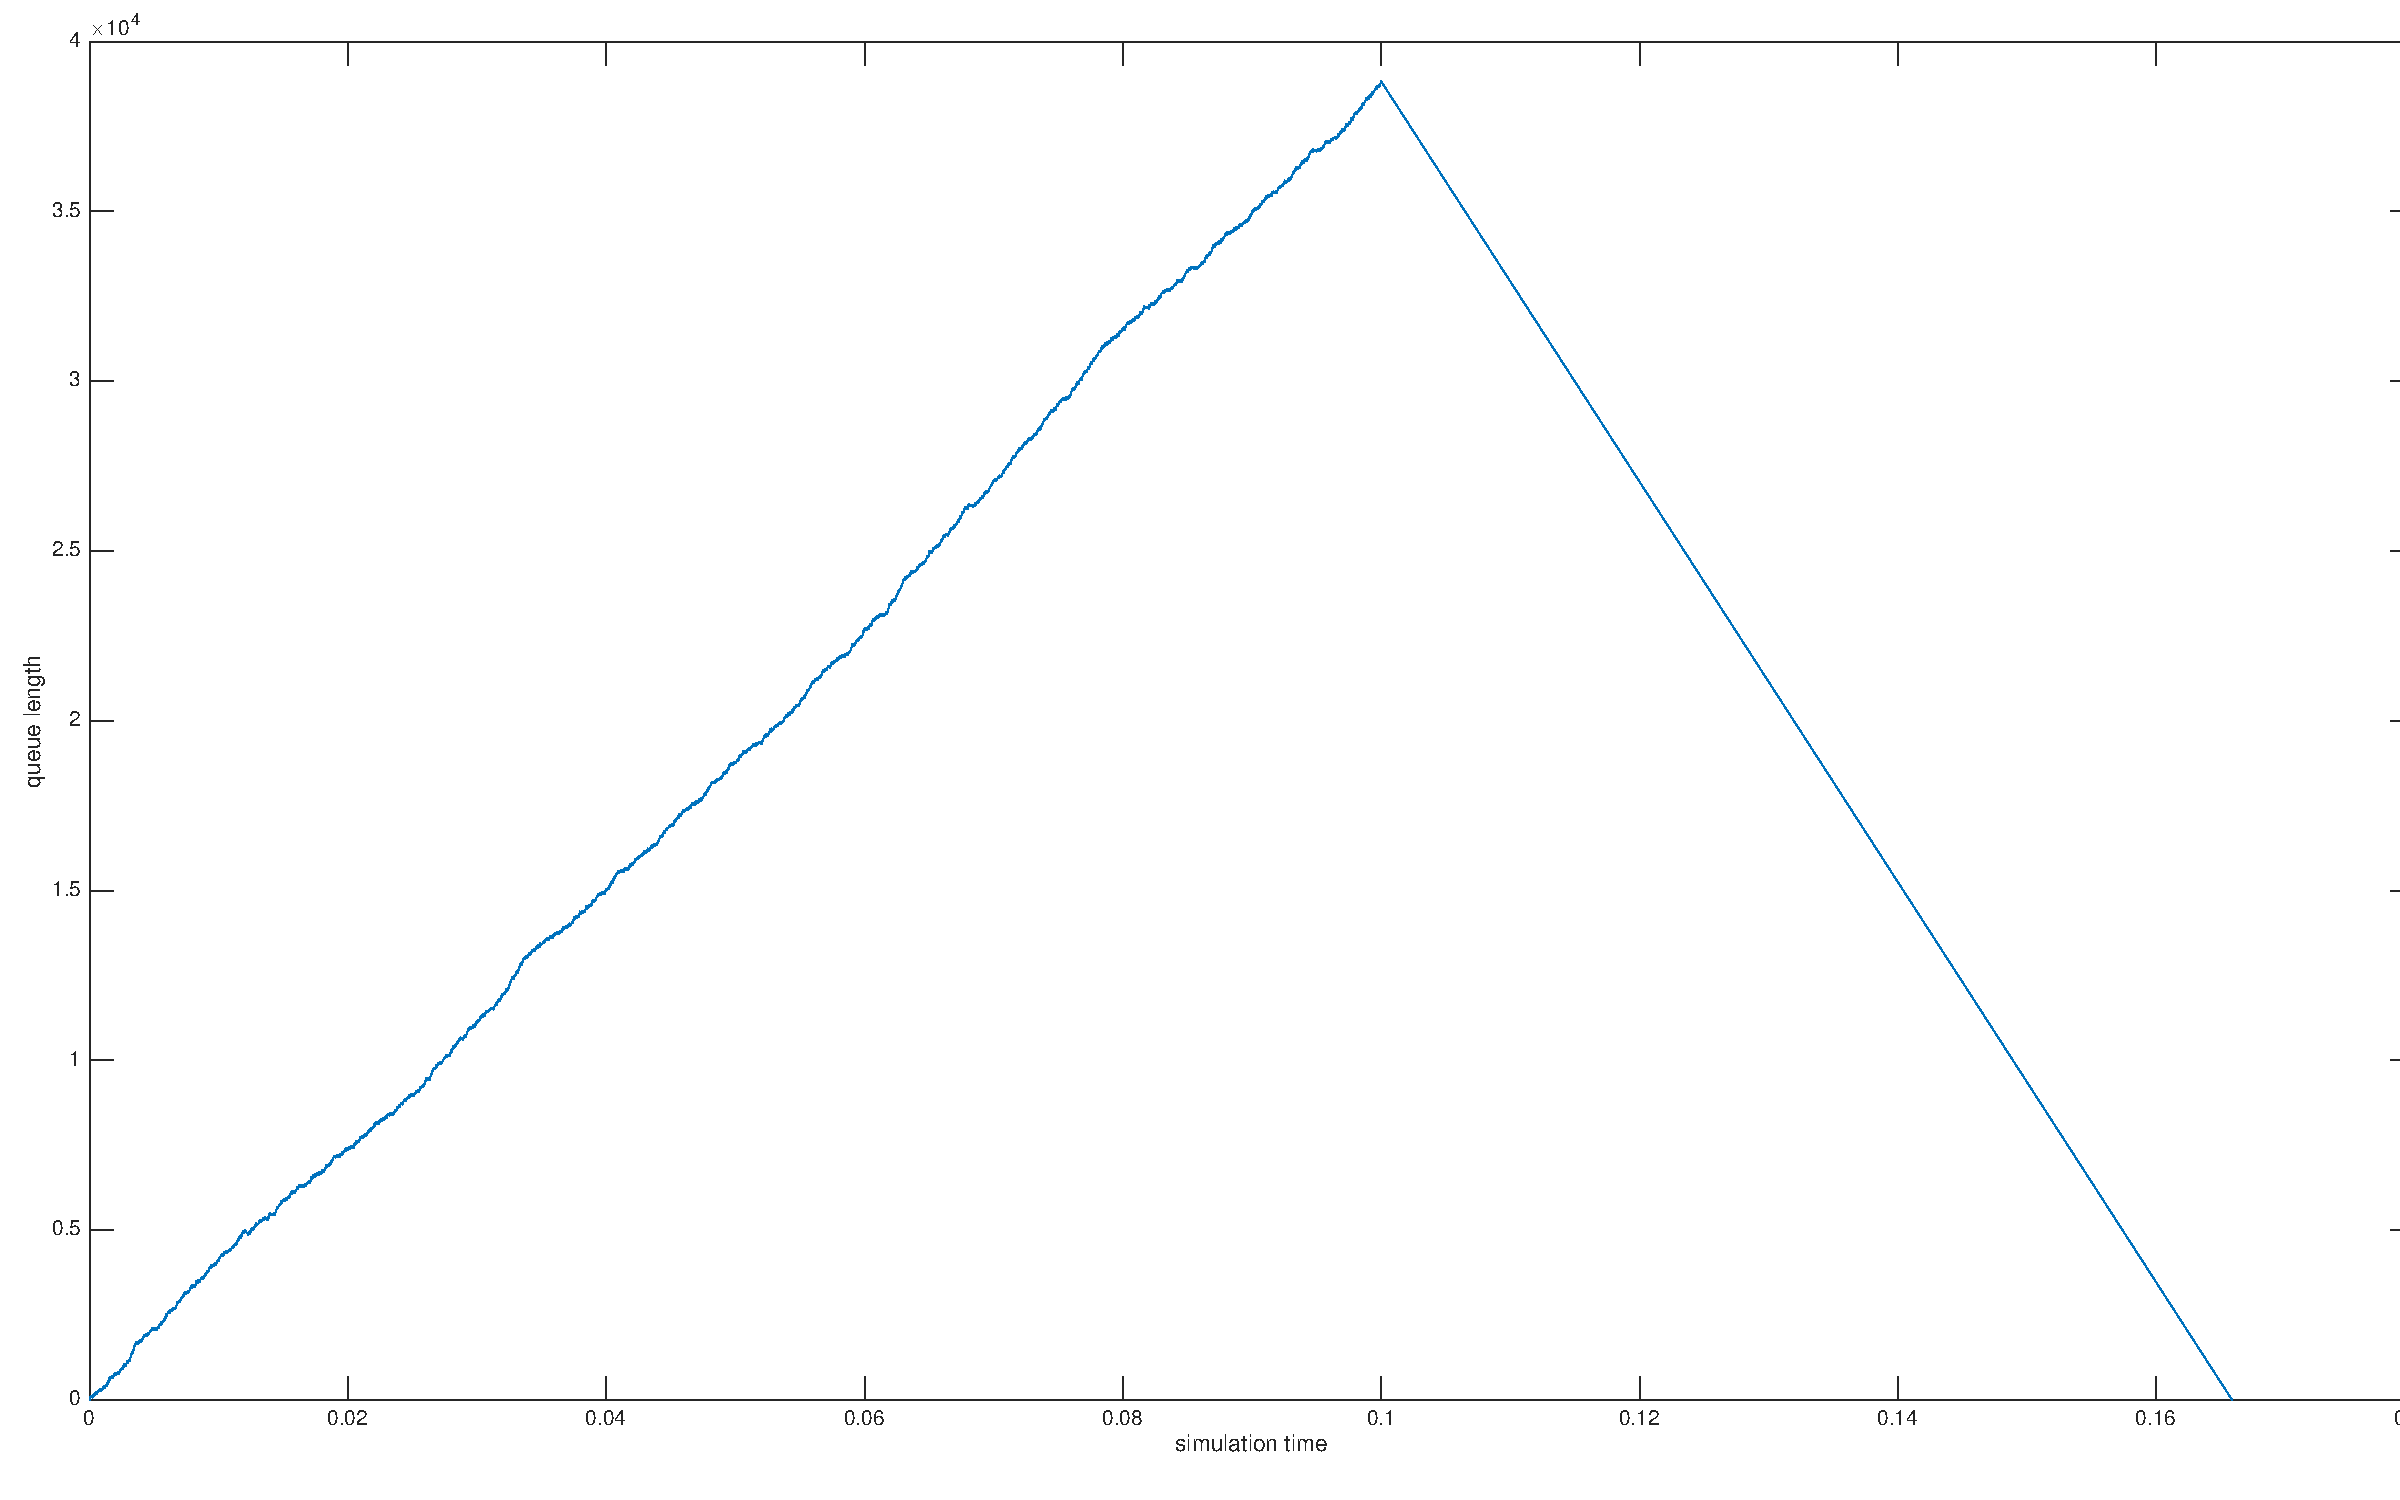
\includegraphics[width=\textwidth]{images/app1-queue2.pdf}
    \caption{Application 1: The number of tasks in the SSO/core queue, from the second resource usage queue.}
    \label{fig:app1-queue2}
  \end{center}
\end{figure}

\begin{figure}[]
  \begin{center}
    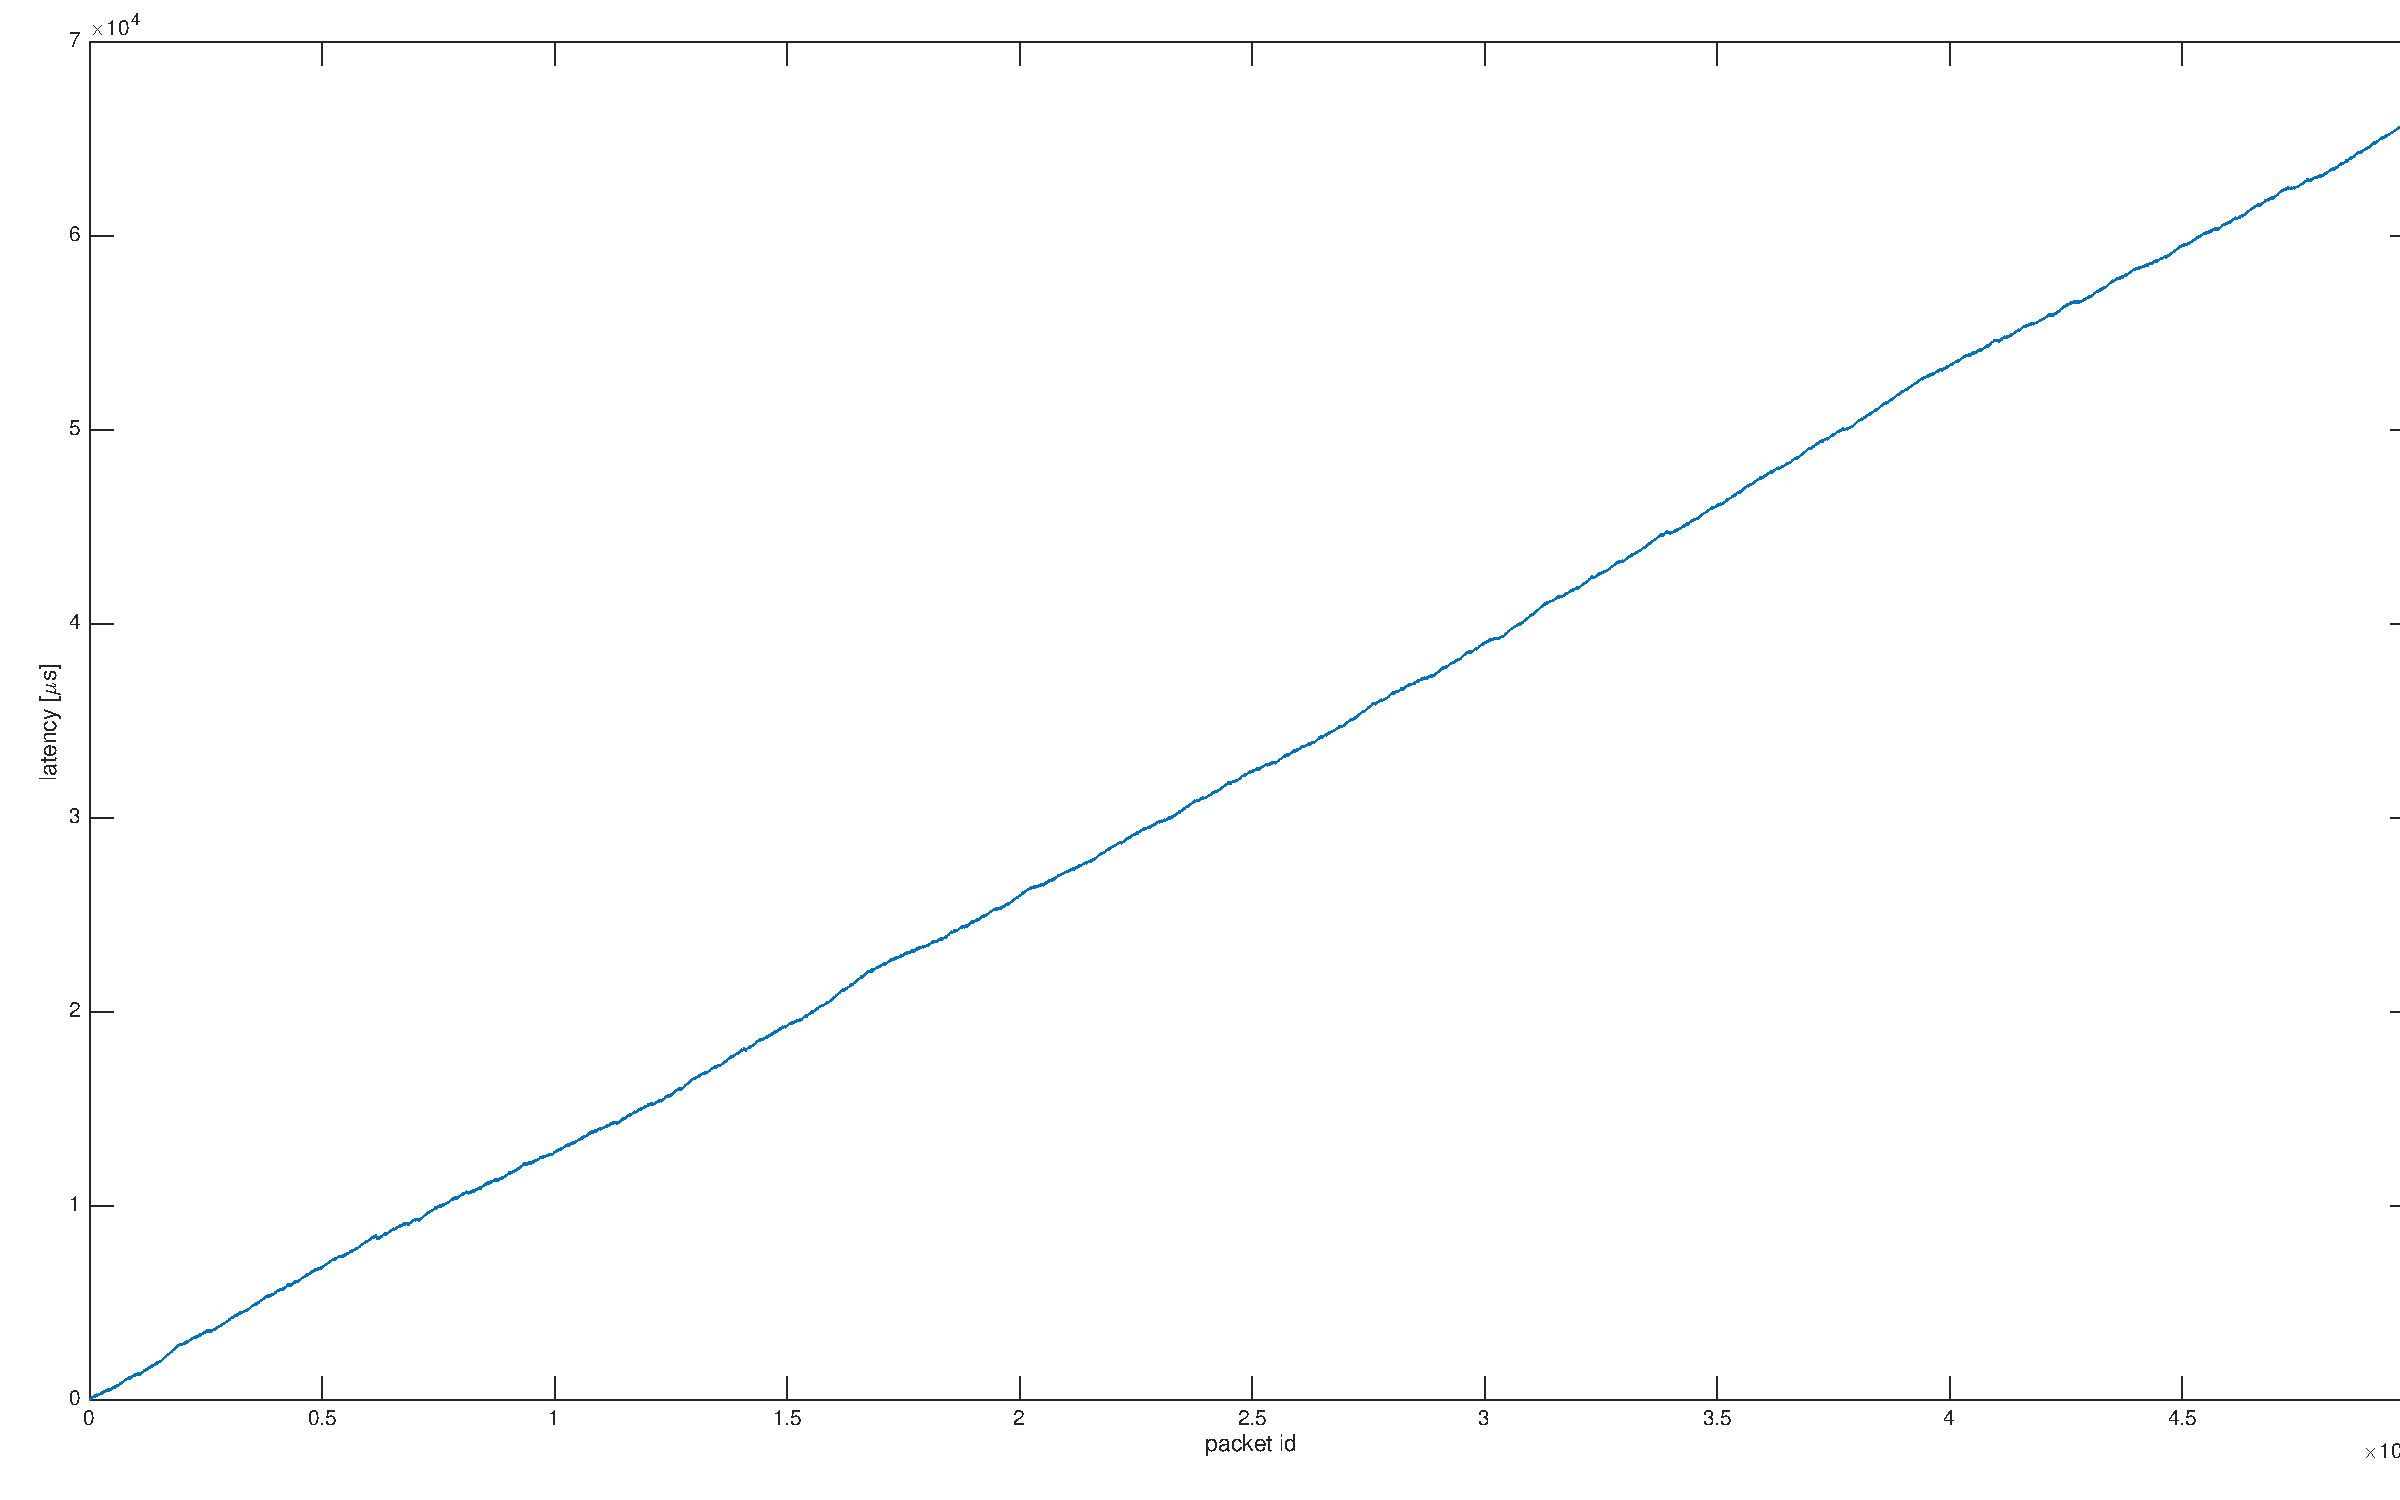
\includegraphics[width=\textwidth]{images/app1-latency.pdf}
    \caption{Application 1: Latency of the packets through the system.}
    \label{fig:app1-latency}
  \end{center}
\end{figure}

It is clear from the figures, that the second processing step is a bottleneck in the system. The processing in the second execution object is so heavy that the tasks accumulate into the waiting queue, and thus the packet latency keeps growing.

The second application removes this problem, by parallelizing part of the atomic processing. Figures~\ref{fig:app2-queue2} and \ref{fig:app2-latency} present the data from the second application simulation. Figure~\ref{fig:app2-queue2} shows the number of tasks in the SSO/core queue, that are from the atomic resource usage queue, with respect to simulation time. Figure~\ref{fig:app2-latency} presents the latency of the packets through the whole system. Neither of the parallel queues have tasks in the waiting queue of the SSO/core during the simulation.

\begin{figure}[]
  \begin{center}
    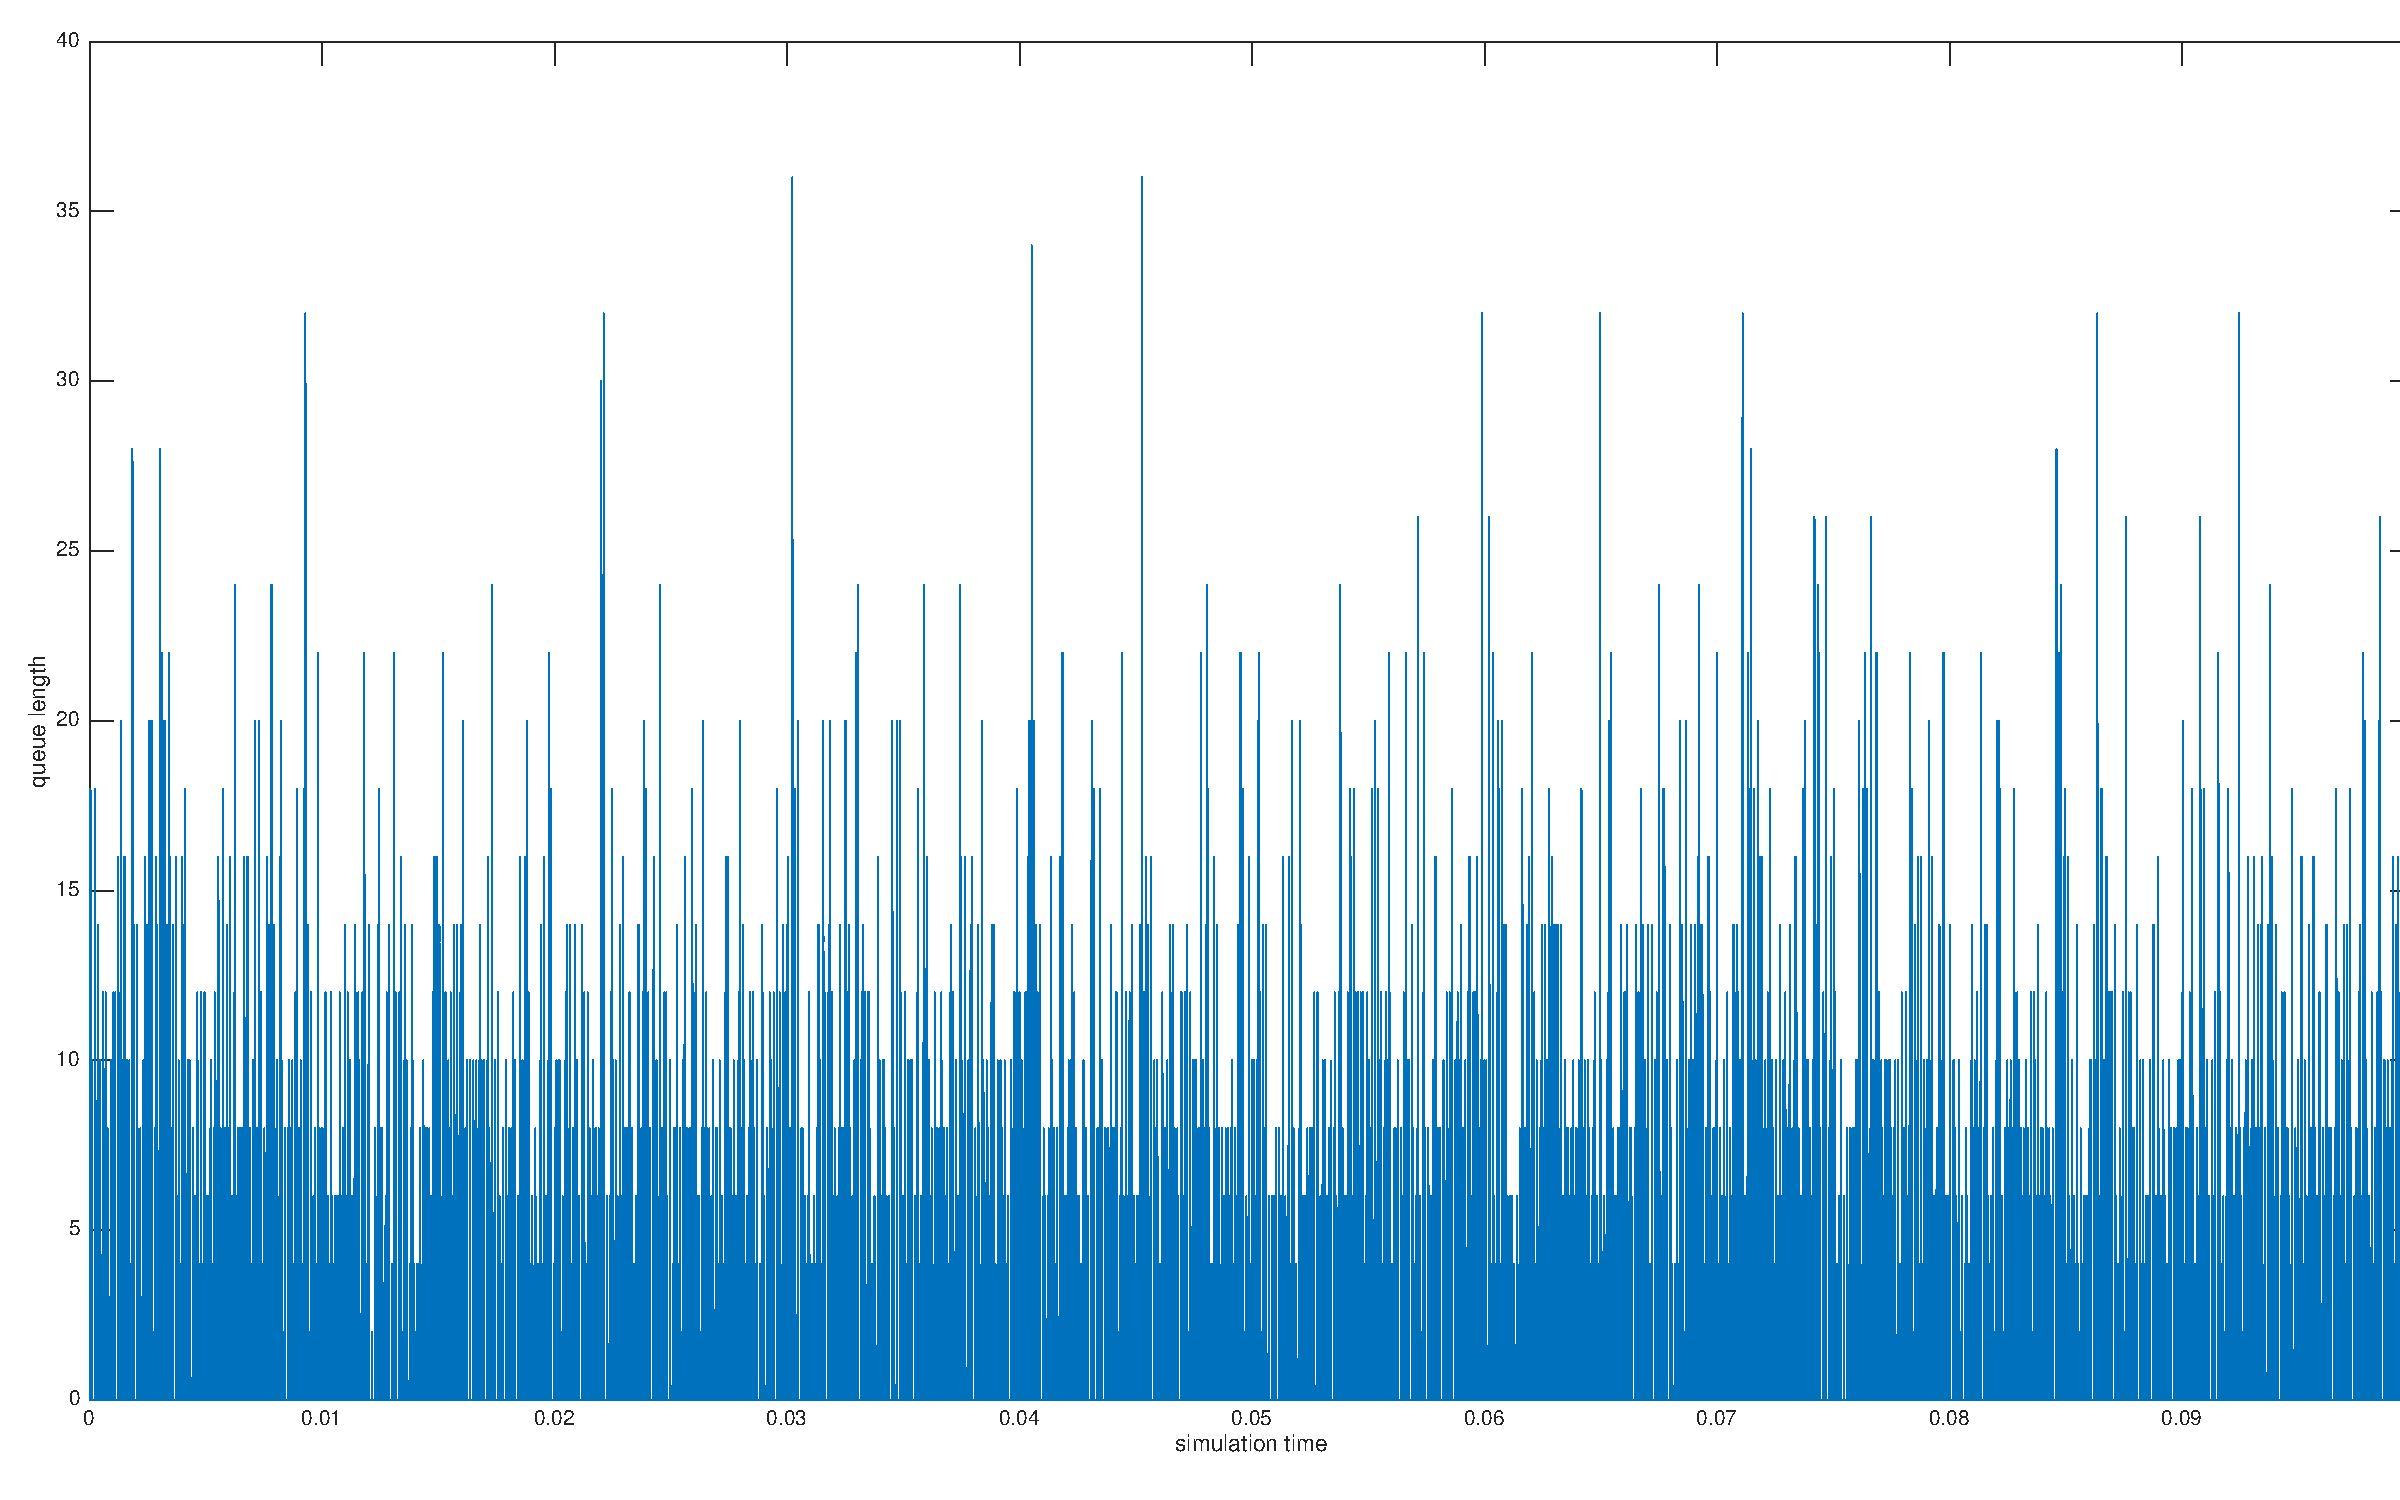
\includegraphics[width=\textwidth]{images/app2-queue2.pdf}
    \caption{Application 2: The number of tasks in the SSO/core queue, from the second resource usage queue.}
    \label{fig:app2-queue2}
  \end{center}
\end{figure}

\begin{figure}[]
  \begin{center}
    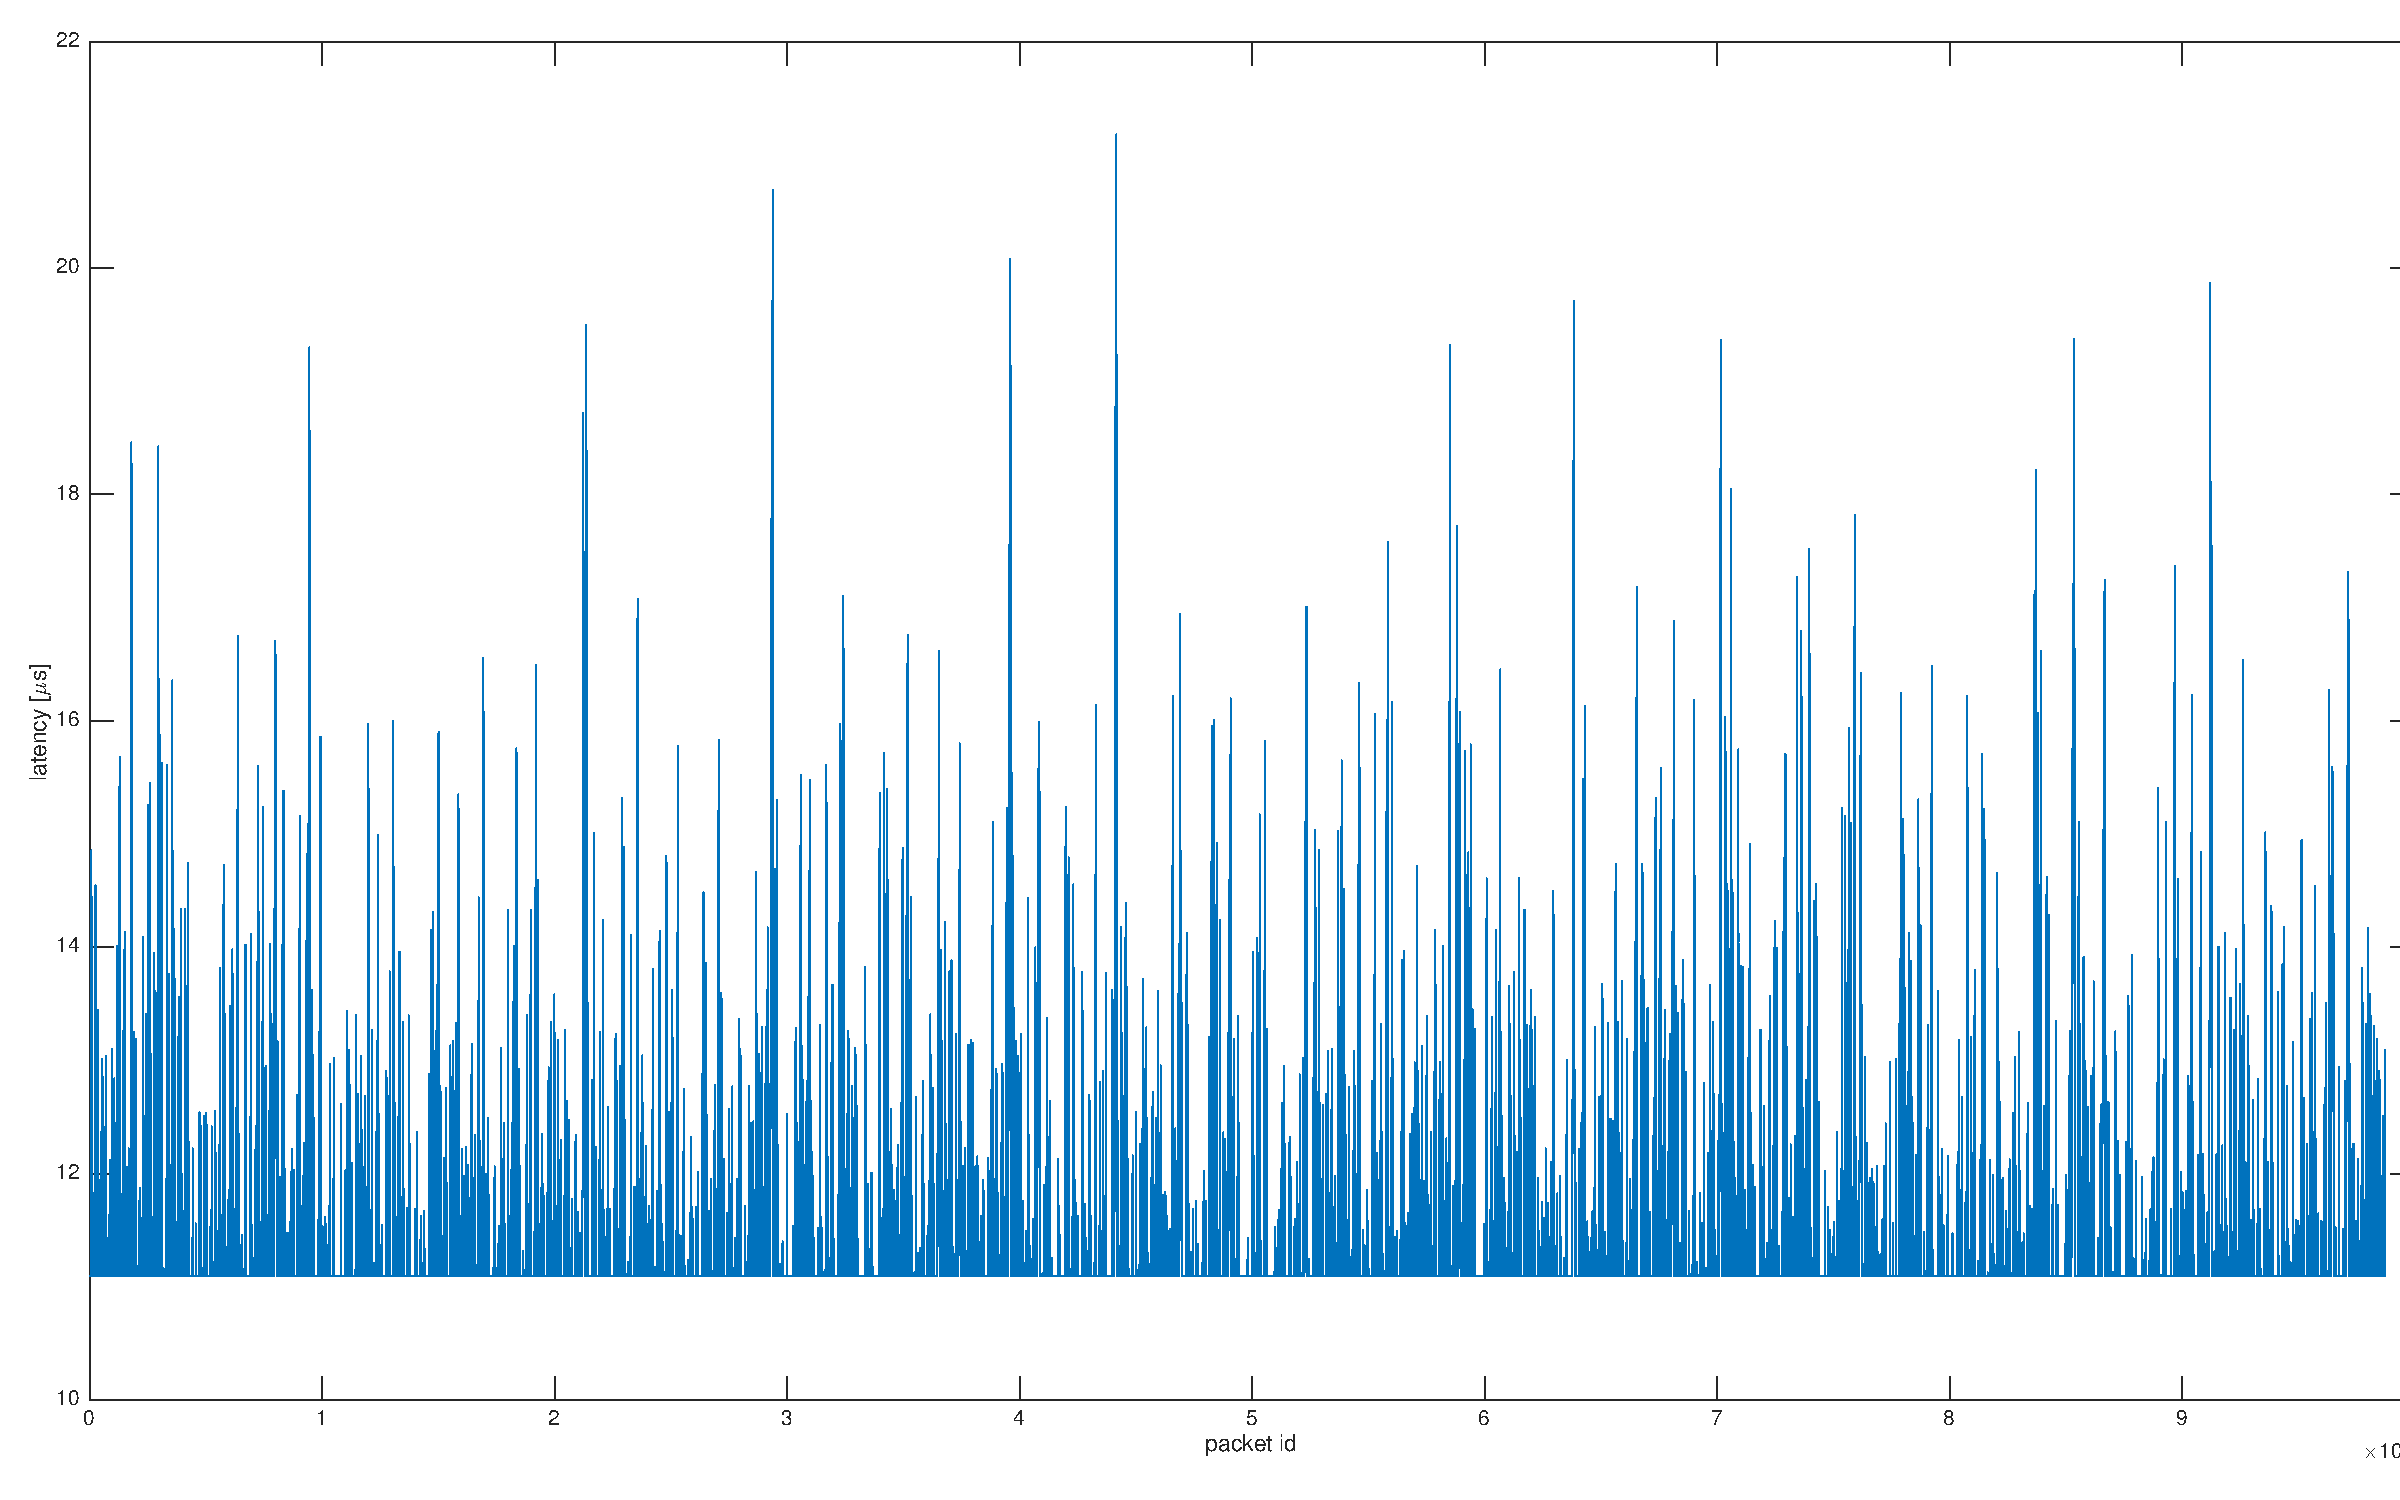
\includegraphics[width=\textwidth]{images/app2-latency.pdf}
    \caption{Application 2: Latency of the packets through the system.}
    \label{fig:app2-latency}
  \end{center}
\end{figure}

As the figures show, the bottleneck is removed from the system, and the latencies stay within 22$\mu$s during the simulation.

\section{Discoveries}

% \section{Building prototype system based on the model}

%%% Local Variables:
%%% mode: latex
%%% TeX-master: "thesis-hartikainen"
%%% End:
